\documentclass[landscape]{beamer}
\usepackage{xcolor}
\usepackage{amsmath, amsthm}
\newtheorem{benchmark}{Benchmark}
\newtheorem{environment}{Environment}
\newtheorem{distribution}{The Distribution of Counting Operators in Our Benchmark}
\usepackage{mathrsfs}
\usepackage{hyperref}
\usepackage{algpseudocode}
\usepackage{tikz}
\usetikzlibrary {decorations.pathmorphing, curvilinear, shadows,shapes.symbols, automata, positioning, shapes,arrows, matrix}
\usepackage{multicol}
\usepackage{pgfplots}
\usepackage{array}
\usepackage{colortbl}
\definecolor{grayshade}{gray}{0.9}
\usepackage{listings}
\lstdefinestyle{myjs}{
  language=C,
  basicstyle=\ttfamily,
  keywordstyle=\color{blue},
  stringstyle=\color{red},
  commentstyle=\color{green},
  backgroundcolor=\color{gray!10},
  breaklines=true,
  frame=single,
  captionpos=b
}
\usepackage{booktabs}
\usepackage{siunitx}
\usepackage{graphicx}

\linespread{1.5}
\newcommand{\aut}{\mathcal{A}}
\newcommand{\myvec}[1]{\overrightarrow{#1}}
\newcommand{\cB}{\mathcal{B}}
\newcommand{\anivar}{\mathfrak{x}}
\newcommand*{\ostrichrecl}{\rm OSTRICH^{RECL}}
\newcommand*{\op}{o}
\newcommand*{\regex}{e}


\colorlet{noteColor}{green!10!orange}

\mode<presentation> {

\usetheme{Singapore}


\useinnertheme{rounded}

\useoutertheme{split}

\usefonttheme{professionalfonts}
}


%------------------------------------------------------------
%This block of code defines the information to appear in the
%Title page
\graphicspath{{pics/}}

\title{String Constraints with Regex-Counting and
String-Length Solved More Efficiently}
\author{\textbf{Denghang Hu}, Zhilin Wu}
% \institute{}

% Add the image inside titlegraphics macro
\titlegraphic{
  \includegraphics[width=0.2\textwidth]{pics/ISCAS-logo.jpeg} \quad\quad\quad\quad
  \includegraphics[width=0.3\textwidth]{pics/ucas_logo.pdf}
}

%End of title page configuration block
%------------------------------------------------------------

%------------------------------------------------------------
%The next block of commands puts the table of contents at the 
%beginning of each section and highlights the current section:

\AtBeginSection[]
{
  \begin{frame}
    \tableofcontents[currentsection]
  \end{frame}
}
%------------------------------------------------------------

\begin{document}

\pdfbookmark{Title}{Title}
%The next statement creates the title page.
\frame{\titlepage}

% no more than 15 mins 
% Introduction : (3min)
% 1 Motivation
% 3 contribution of our work (overview)
\section{Introduction}

\begin{frame}{Strings are Important}
  \textbf{Strings are primitive in program languages:}
  \begin{itemize}
    \item C/C++/C\#
    \item Java
    \item JavaScript/TypeScript
    \item Python
    \item Go
  \end{itemize}
\end{frame}

\begin{frame}{Strings are Widely Used in Security-Critical Situations\footnote{Tevfik Bultan, et al.: String Analysis for Software Verification and Security.}}
  \begin{itemize}
    \item Input sanitisation, validation
    \item Quary generation for databases
    \item Data handling: XML, JSON, HTML
    \item Dynamic code generation
  \end{itemize}
\end{frame}


\begin{frame}
  \frametitle{Strings Are Error-Prone}
  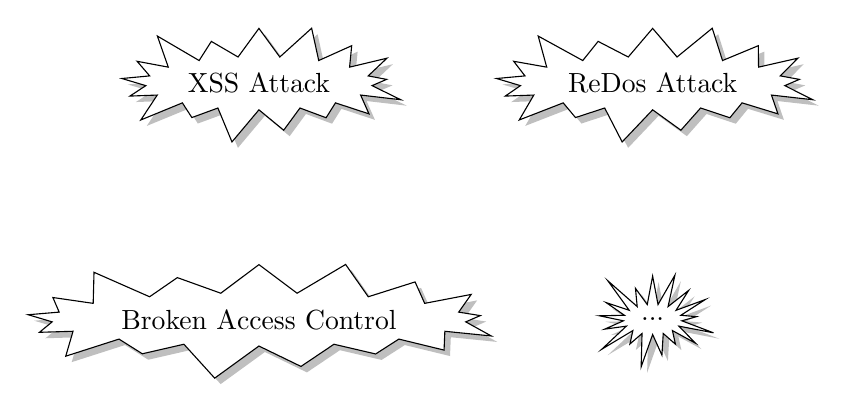
\begin{tikzpicture}
    \node[starburst,drop shadow,fill=white,draw] at (0,0) {XSS Attack};
    \node[starburst,drop shadow,fill=white,draw] at (5,0) {ReDos Attack};
    \node[starburst,drop shadow,fill=white,draw] at (0,-3) {Broken Access Control};
    \node[starburst,drop shadow,fill=white,draw] at (5,-3) {...};
  \end{tikzpicture}
\end{frame}

\begin{frame}[fragile]{Detect Attacks by String Constraints}
  \textbf{Malicious User Input:}
  \begin{lstlisting}[style=myjs]
      <script> XSSAtack </script>
    \end{lstlisting}
  \textbf{Detect the Attack by String Constraints:}
  \begin{lstlisting}[style=myjs]
    (assert (str.contains x '<script>'))
  \end{lstlisting}
\end{frame}

\begin{frame}
  \frametitle{String Solvers}
  \begin{multicols}{2}
    \begin{itemize}
      \item ABC
      \item \textbf{CVC3/4/5}
      \item Gecode+S
      \item \textbf{OSTRICH}
      \item Stranger
      \item S3/p/\#
      \item Sloth
      \item SLENT
      \item TRAU/+
      \item Woorpje
      \item \textbf{Z3str2/3/4/RE/Seq}
      \item ...
    \end{itemize}
  \end{multicols}
\end{frame}


\begin{frame}{Motivation Example}
  \textbf{CVC5 and Z3 Cannot Solve:}
  \begin{tikzpicture}
    \node (formula) at (0,0) {
    $
      x\in (\Sigma \backslash a)^{\textcolor{red}{\{1,60\}}}(\Sigma \backslash b)^{\textcolor{red}{\{1,60\}}}(\Sigma \backslash c)^{\textcolor{red}{\{0,60\}}} \wedge x\in \Sigma^*c^+ \wedge \textcolor{red}{|x|} > 120
    $
    };
    \node [rotate=45, scale=2, text=red!90, fill=yellow!20,draw,decorate,decoration={bumps,mirror}, opacity=0] at (1,0) {300s TIMEOUT};
  \end{tikzpicture}
\end{frame}
\begin{frame}{Motivation Example}
  \textbf{CVC5 and Z3 Cannot Solve:}
  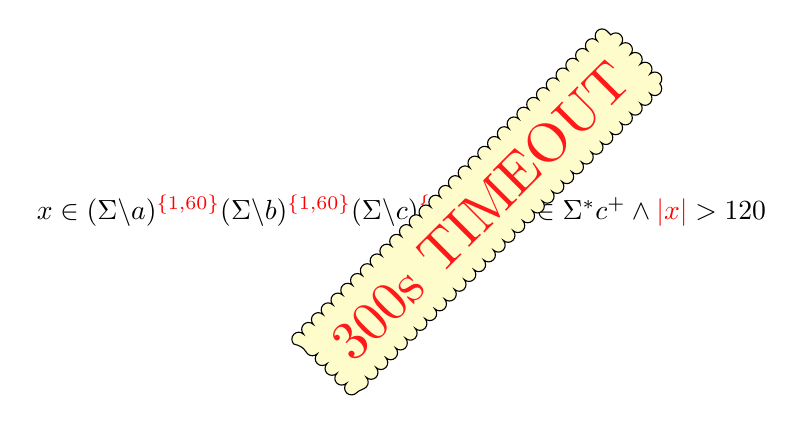
\begin{tikzpicture}
    \node (formula) at (0,0) {
    $
      x\in (\Sigma \backslash a)^{\textcolor{red}{\{1,60\}}}(\Sigma \backslash b)^{\textcolor{red}{\{1,60\}}}(\Sigma \backslash c)^{\textcolor{red}{\{0,60\}}} \wedge x\in \Sigma^*c^+ \wedge \textcolor{red}{|x|} > 120
    $
    };
    \node [rotate=45, scale=2, text=red!90, fill=yellow!20,draw,decorate,decoration={bumps,mirror}] at (1,0) {300s TIMEOUT};
  \end{tikzpicture}
\end{frame}


\begin{frame}[fragile]
  \frametitle{However ...}
  \textbf{Regex-Countings are Widely Used}
  \begin{table}
    \centering
    \begin{tabular}{l l l S[table-format=1.2]}
      \toprule
      \textbf{Rank} & \textbf{Type}  & \textbf{Example} & \textbf{\% Projects} \\
      \midrule
      1             & $\cdot\{1,\}$  & $z^+$            & 73.2                 \\
      3             & $\cdot\{0,\}$  & $z^*$            & 66.8                 \\
      18            & $\cdot\{n\}$   & $z\{8\}$         & 20.7                 \\
      20            & $\cdot\{n,m\}$ & $z\{8,9\}$       & 14.5                 \\
      \bottomrule
    \end{tabular}
    \caption{The Rank and Percentage of Regex-Countings in Python \footnote{Chapman,C. et al: Exploring regular expression usage and context in python}}
  \end{table}

\end{frame}

\begin{frame}[fragile]
  \frametitle{However ...}
  \textbf{String-Length is Widely Used}
  \begin{figure}
    \includegraphics[width=.5\linewidth]{length_percentage.jpg}
    \caption{The Percentages of String Operations in Web Applications \footnote{Saxena, P. et al: A symbolic execution framework for JavaScript.}}
  \end{figure}
\end{frame}

% Technical details : (8min)
% 1 What is Regex-Counting
% 2 normal ways (z3, cvc5, trau)
% 3 our ways
%   1 An example (5-7 pages)
%   2 Decisino procedure 1 pages
\section{Our Approach}
\begin{frame}{The Problem}
  Syntax of \textbf{RE}gex-\textbf{C}ounting \textbf{L}ogic (\textbf{RECL}):
  \begin{figure}[h]
    \centering
    \resizebox{1\linewidth}{!}{
      $
        \begin{array}{l l l l}
          \varphi & ::= & x\in \regex \mid t_1\  \op\ t_2 \mid  \varphi \wedge \varphi                                                                                         & \mbox{formulas}      \\
          \regex  & ::= & \emptyset \mid \epsilon \mid a \mid \regex\cdot \regex \mid \regex+\regex \mid \regex^* \mid \regex \cap \regex \mid                                 &                      \\
                  &     & \overline{\regex} \mid \regex \setminus \regex \mid {\textcolor{red!90}{\regex^{\{m,n\}}}} \mid {\textcolor{red!90}{\regex^{\{m,\infty\}}}} \mid (e) & \mbox{regexes}       \\
          t       & ::= & n \mid \anivar \mid  {\textcolor{red!90}{|x|}} \mid t - t \mid t + t                                                                                 & \mbox{integer terms}
        \end{array}
      $
    }
  \end{figure}
\end{frame}
\begin{frame}{Motivation Example}
  \begin{tikzpicture}
    \node (placeholder) at (0,0) {
    $
      x\in (\Sigma \backslash a)^{\textcolor{red}{\{1,60\}}}(\Sigma \backslash b)^{\textcolor{red}{\{1,60\}}}(\Sigma \backslash c)^{\textcolor{red}{\{0,60\}}} \wedge x\in \Sigma^*c^+ \wedge \textcolor{red}{|x|} > 120
    $
    };
    \node [rotate=45, scale=2, text=red!90, fill=yellow!20,draw,decorate,decoration={bumps,mirror}, opacity=0] at (1,0) {300s TIMEOUT};
  \end{tikzpicture}
\end{frame}

\begin{frame}[fragile]{Exsiting Techniques to Solve Such Constraints}
  \begin{minipage}{0.48\linewidth}
    \begin{tikzpicture}
      \node [anchor=west, align=left, text width = .9\linewidth] (text) at (0,-2) {
        Rule-based (CVC5, Z3): \\ \textbf{Repeatly unwind} counting operators by derivation rules.
      };
      \node [anchor=west, align=left] (cvc5) at (0,-4) {
        \includegraphics[width=0.4\linewidth]{cvc5_logo.png}
      };
      \node [anchor=west, align=left] (z3) at (3,-4) {
        \includegraphics[width=0.2\linewidth]{Z3_logo.jpeg}
      };
      \node [anchor=west, align=left] (example) at (0,-5.5) {$a^{\{1,3\}}: a, aa, aaa$};
      \node [anchor=west, align=left,rotate=45, scale=1.5, text=red!90, fill=yellow!20,draw,decorate,decoration={bumps,mirror}, opacity = 0] at (0,-5.5) {Exponential Search Space};
    \end{tikzpicture}
  \end{minipage}
  \begin{minipage}{0.48\linewidth}
    \begin{tikzpicture}
      \node [anchor=west, align=left, text width = \linewidth] (text) at (0,-2) {
        Automaton-based (Z3Str3RE, OSTRICH):\textbf{Unwind} counting operators before constructing automata.
      };
      \node [anchor = west, align=center] (z3) at (3,-4) {
        \includegraphics[width=0.25\linewidth]{ostrich_logo.jpeg}
      };
      \node [anchor = west, align=left, rotate=45, scale=1.5, text=red!90, fill=yellow!20,draw,decorate,decoration={bumps,mirror}, opacity = 0] at (0,-4) {State Explosion};
      \node [anchor=west, align=left] (example) at (0,-5.5) {
        \begin{tikzpicture}[node distance=0.5cm, auto,semithick, initial text=$a^{\{1,3\}}:$,
            every state/.style={inner sep=1pt, minimum size=5pt}]
          \node[state,initial] (q0) {$q_0$};
          \node[state, accepting] (q1) [right=of q0] {$q_1$};
          \node[state, accepting] (q2) [right=of q1] {$q_2$};
          \node[state, accepting] (q3) [right=of q2] {$q_3$};
          \path[->]
          (q0) edge [above] node {$a$} (q1)
          (q1) edge [above] node {$a$} (q2)
          (q2) edge [above] node {$a$} (q3);
        \end{tikzpicture}
      };
    \end{tikzpicture}
  \end{minipage}
\end{frame}
\begin{frame}[fragile]{Exsiting Techniques to Solve Such Constraints}
  \begin{minipage}{0.48\linewidth}
    \begin{tikzpicture}
      \node [anchor=west, align=left, text width = .9\linewidth] (text) at (0,-2) {
        Rule-based (CVC5, Z3): \\ \textbf{Repeatly unwind} counting operators by derivation rules.
      };
      \node [anchor=west, align=left] (cvc5) at (0,-4) {
        \includegraphics[width=0.4\linewidth]{cvc5_logo.png}
      };
      \node [anchor=west, align=left] (z3) at (3,-4) {
        \includegraphics[width=0.2\linewidth]{Z3_logo.jpeg}
      };
      \node [anchor=west, align=left] (example) at (0,-5.5) {$a^{\{1,3\}}: a, aa, aaa$};
      \node [anchor=west, align=left,rotate=45, scale=1.5, text=red!90, fill=yellow!20,draw,decorate,decoration={bumps,mirror}] at (0,-5.5) {Exponential Search Space};
    \end{tikzpicture}
  \end{minipage}
  \begin{minipage}{0.48\linewidth}
    \begin{tikzpicture}
      \node [anchor=west, align=left, text width = \linewidth] (text) at (0,-2) {
        Automaton-based (Z3Str3RE, OSTRICH):\textbf{Unwind} counting operators before constructing automata.
      };
      \node [anchor = west, align=center] (z3) at (3,-4) {
        \includegraphics[width=0.25\linewidth]{ostrich_logo.jpeg}
      };
      \node [anchor = west, align=left, rotate=45, scale=1.5, text=red!90, fill=yellow!20,draw,decorate,decoration={bumps,mirror}] at (0,-4) {State Explosion};
      \node [anchor=west, align=left] (example) at (0,-5.5) {
        \begin{tikzpicture}[node distance=0.5cm, auto,semithick, initial text=$a^{\{1,3\}}:$,
            every state/.style={inner sep=1pt, minimum size=5pt}]
          \node[state,initial] (q0) {$q_0$};
          \node[state, accepting] (q1) [right=of q0] {$q_1$};
          \node[state, accepting] (q2) [right=of q1] {$q_2$};
          \node[state, accepting] (q3) [right=of q2] {$q_3$};
          \path[->]
          (q0) edge [above] node {$a$} (q1)
          (q1) edge [above] node {$a$} (q2)
          (q2) edge [above] node {$a$} (q3);
        \end{tikzpicture}
      };
    \end{tikzpicture}
  \end{minipage}
\end{frame}

% \begin{frame}{Our Techniques to Such Constraints}
%   \begin{itemize}
%     \item Automata with integer registers
%     \item Encode counting operators by registers (no explicitly unwind)
%     \item Size reduction techniques for automata
%   \end{itemize}
% \end{frame}

\begin{frame}[fragile]{The Main Idea of Our Approach}
  \linespread{0.9}
  \begin{tikzpicture}[anchor=west]
    \node (a_1_3) at (0, 0) {
      \begin{tikzpicture}[node distance=0.5cm, auto,semithick, initial text=$a^{\{1,3\}}:$,
          every state/.style={inner sep=1pt, minimum size=5pt}]
        \node[state,initial] (q0) {$q_0$};
        \node[state, accepting] (q1) [right=of q0] {$q_1$};
        \node[state, accepting] (q2) [right=of q1] {$q_2$};
        \node[state, accepting] (q3) [right=of q2] {$q_3$};
        \path[->]
        (q0) edge [above] node {$a$} (q1)
        (q1) edge [above] node {$a$} (q2)
        (q2) edge [above] node {$a$} (q3);
      \end{tikzpicture}
    };
    \node (text1) at (6,0) {\textbf{Finite Automata}};
    \node (a_1_3_cefa) at (0,-1.5) {
      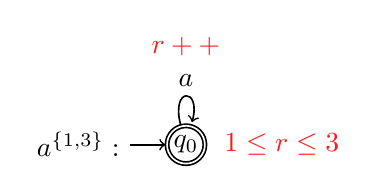
\begin{tikzpicture}[node distance=0.1cm, auto,semithick,  initial text=$a^{\{1,3\}}:$,
          every state/.style={inner sep=1pt, minimum size=5pt}]
        \node[state,initial,accepting] (q0) {$q_0$};
        \node (accepting_condition) [right=of q0] {$\textcolor{red!90}{1\leq r\leq3}$};
        \path[->]
        (q0) edge [loop above] node [align=center] {$\textcolor{red!90}{r++}$ \\ $a$} (q0);
      \end{tikzpicture}
    };
    \node [align=center] (text2) at (5,-3.25) {\textbf{Cost-Enriched Finite Automata}\\\textbf{(CEFA)}};
    \node (a_len) at (0, -4) {
      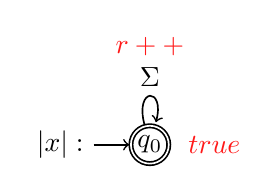
\begin{tikzpicture}[node distance=0.1cm, auto,semithick,  initial text=$|x|:$,
          every state/.style={inner sep=1pt, minimum size=5pt}]
        \node[state,initial,accepting] (q0) {$q_0$};
        \node (accepting_condition) [right=of q0] {$\textcolor{red!90}{true}$};
        \path[->]
        (q0) edge [loop above] node [align=center] {$\textcolor{red!90}{r++}$ \\ $\Sigma$} (q0);
      \end{tikzpicture}
    };

  \end{tikzpicture}
\end{frame}

\begin{frame}{$ x\in \textcolor{red!90}{(\Sigma \backslash a)^{\{1,60\}}(\Sigma \backslash b)^{\{1,60\}}(\Sigma \backslash c)^{\{0,60\}}} \wedge x\in \Sigma^*c^+ \wedge |x| > 120$}
  \textbf{1. Encode Counting Operators and Lengths by CEFAs }
  \begin{figure}
    \includegraphics[width=\linewidth]{overview_regex1.jpg}
  \end{figure}
\end{frame}
\begin{frame}{$ x\in (\Sigma \backslash a)^{\{1,60\}}(\Sigma \backslash b)^{\{1,60\}}(\Sigma \backslash c)^{\{0,60\}} \wedge x\in \textcolor{red!90}{\Sigma^*c^+} \wedge |x| > 120$}
  \textbf{1. Encode Counting Operators and Lengths by CEFAs }
  \begin{figure}
    \includegraphics[width=.5\linewidth]{overview_regex2.jpg}
  \end{figure}
\end{frame}
\begin{frame}{$ x\in (\Sigma \backslash a)^{\{1,60\}}(\Sigma \backslash b)^{\{1,60\}}(\Sigma \backslash c)^{\{0,60\}} \wedge x\in \Sigma^*c^+ \wedge \textcolor{red!90}{|x|} > 120$}
  \textbf{1. Encode Counting Operators and Lengths by CEFAs}
  \begin{figure}
    \includegraphics[width=.25\linewidth]{overview_length_pre.jpg}
  \end{figure}
\end{frame}


\begin{frame}{$ x\in (\Sigma \backslash a)^{\{1,60\}}(\Sigma \backslash b)^{\{1,60\}}(\Sigma \backslash c)^{\{0,60\}} \wedge x\in \Sigma^*c^+ \wedge |x| > 120$}
  \textbf{2. Compute the Product of CEFAs }
  \begin{figure}
    \includegraphics[width=.65\linewidth]{overview_product.jpg}
  \end{figure}
\end{frame}
\begin{frame}{$ x\in (\Sigma \backslash a)^{\{1,60\}}(\Sigma \backslash b)^{\{1,60\}}(\Sigma \backslash c)^{\{0,60\}} \wedge x\in \Sigma^*c^+ \wedge \textcolor{red}{|x| > 120}$}
  \textbf{2. Compute the Product of CEFAs }
  \begin{tikzpicture}
    \node (product) at (0,0) {
      \includegraphics[width=.65\linewidth]{overview_product.jpg}
    };
    \node (lia) at (6,0) {
      $\textcolor{red}{r_4 > 120}$
    };
  \end{tikzpicture}
\end{frame}
\begin{frame}{$ x\in (\Sigma \backslash a)^{\{1,60\}}(\Sigma \backslash b)^{\{1,60\}}(\Sigma \backslash c)^{\{0,60\}} \wedge x\in \Sigma^*c^+ \wedge \textcolor{red}{|x| > 120}$}
  \textbf{2. Compute the Product of CEFAs }
  \begin{tikzpicture}
    \node (product) at (0,0) {
      \includegraphics[width=.65\linewidth]{overview_product.jpg}
    };
    \node (lia) at (6,0) {
      $\textcolor{red}{r_4 > 120}$
    };
    \node (nonempty) [scale=1.3, text=blue!60, fill=yellow!20,draw,decorate,decoration={bumps,mirror}] at (2, 0) {The Nonemptiness of CEFA w.r.t LIA Formulas};
  \end{tikzpicture}
\end{frame}
\begin{frame}{$ x\in (\Sigma \backslash a)^{\{1,60\}}(\Sigma \backslash b)^{\{1,60\}}(\Sigma \backslash c)^{\{0,60\}} \wedge x\in \Sigma^*c^+ \wedge \textcolor{red}{|x| > 120}$}
  \textbf{2. Compute the Product of CEFAs }
  \begin{tikzpicture}
    \node (product) at (0,0) {
      \includegraphics[width=.65\linewidth]{overview_product.jpg}
    };
    \node (lia) at (6,0) {
      $\textcolor{red}{r_4 > 120}$
    };
    \node (nonempty) [scale=1.3, text=blue!60, fill=yellow!20,draw,decorate,decoration={bumps,mirror}] at (2, 0) {The Nonemptiness of CEFA w.r.t LIA Formulas};
    \node (satisfy) [scale=1.3, text=red!60, fill=yellow!20,draw,decorate,decoration={bumps,mirror}] at (2, -2) {The Satisfiability of LIA Formulas};
    \draw [->, line width=4pt, orange!100, -triangle 90] (nonempty) -- (satisfy);
  \end{tikzpicture}
\end{frame}


\begin{frame}{$ x\in (\Sigma \backslash a)^{\{1,60\}}(\Sigma \backslash b)^{\{1,60\}}(\Sigma \backslash c)^{\{0,60\}} \wedge x\in \Sigma^*c^+ \wedge |x| > 120$}
  3. Reduce the Nonemptiness of CEFA w.r.t. LIA formulas to the Satisfiability of LIA Formulas: \textbf{Size-Reduction Techniques}
  \begin{figure}
    \includegraphics[width=.55\linewidth]{overview_product_vector.jpg}
  \end{figure}
\end{frame}

\begin{frame}[fragile]{$ x\in (\Sigma \backslash a)^{\{1,60\}}(\Sigma \backslash b)^{\{1,60\}}(\Sigma \backslash c)^{\{0,60\}} \wedge x\in \Sigma^*c^+ \wedge |x| > 120$}
  3. Reduce the Nonemptiness of CEFA w.r.t. LIA formulas to the Satisfiability of LIA Formulas: \textbf{Size-Reduction Techniques}
  \begin{tikzpicture}
    \node (B) at (0,0) {$\cB$};
    \node (simplify) [right=of B] {\includegraphics[width=.4\linewidth]{overview_product_vector_simplify.jpg}};
    \node [align=left, text width = .9\linewidth] (size-reduct)  [right=of simplify] {\textcolor{red!60}{\textbf{Determination \\ Minimization}}};
  \end{tikzpicture}
\end{frame}

\begin{frame}{$ x\in (\Sigma \backslash a)^{\{1,60\}}(\Sigma \backslash b)^{\{1,60\}}(\Sigma \backslash c)^{\{0,60\}} \wedge x\in \Sigma^*c^+ \wedge |x| > 120$}
  \textbf{3. Reduce the Nonemptiness of CEFA w.r.t. LIA formulas to the Satisfiability of LIA Formulas}
  \begin{equation*}\label{eqn-LIA}
    \begin{array}{l}
      \textcolor{red!90}{\psi_\cB(\anivar_1, \cdots, \anivar_m)} \wedge \bigwedge \limits_{1 \le j \le 4} \textcolor{blue!90}{ r_j = \sum \limits_{1\le k \le m}  \anivar_k v_{k, j}}\ \wedge \\
      \textcolor{orange!90}{1 \le r_1 \le 60 \wedge 1 \le r_2 \le 60 \wedge 0 \le r_3 \le 60 \wedge r_4 > 120}.
    \end{array}
  \end{equation*}
  \begin{tikzpicture}
    \node [opacity = 0] (placeholder) at (0,0) { \textbf{4. Solve the Parikh Images by the Off-the-Shelf SMT Solver } };
    \node [rotate=45, scale=1.8, text=green!90!black, fill=yellow!20,draw,decorate,decoration={bumps,mirror}, opacity = 0] at (0,0) {1s SOLVED!!!};
  \end{tikzpicture}
\end{frame}
\begin{frame}{$ x\in (\Sigma \backslash a)^{\{1,60\}}(\Sigma \backslash b)^{\{1,60\}}(\Sigma \backslash c)^{\{0,60\}} \wedge x\in \Sigma^*c^+ \wedge |x| > 120$}
  \textbf{3. Reduce the Nonemptiness of CEFA w.r.t. LIA formulas to the Satisfiability of LIA Formulas}
  \begin{equation*}\label{eqn-LIA}
    \begin{array}{l}
      \textcolor{red!90}{\psi_\cB(\anivar_1, \cdots, \anivar_m)} \wedge \bigwedge \limits_{1 \le j \le 4} \textcolor{blue!90}{ r_j = \sum \limits_{1\le k \le m}  \anivar_k v_{k, j}}\ \wedge \\
      \textcolor{orange!90}{1 \le r_1 \le 60 \wedge 1 \le r_2 \le 60 \wedge 0 \le r_3 \le 60 \wedge r_4 > 120}.
    \end{array}
  \end{equation*}
  
\begin{tikzpicture}
    \node (placeholder) at (0,0) { \textbf{4. Solve the LIA Formulas by the Off-the-Shelf SMT Solver } };
    \node [rotate=45, scale=1.8, text=green!90!black, fill=yellow!20,draw,decorate,decoration={bumps,mirror}, opacity = 0] at (0,0) {1s SOLVED!};
  \end{tikzpicture}
\end{frame}
\begin{frame}{$ x\in (\Sigma \backslash a)^{\{1,60\}}(\Sigma \backslash b)^{\{1,60\}}(\Sigma \backslash c)^{\{0,60\}} \wedge x\in \Sigma^*c^+ \wedge |x| > 120$}
  \textbf{3. Reduce the Nonemptiness of CEFA w.r.t. LIA formulas to the Satisfiability of LIA Formulas}
  \begin{equation*}\label{eqn-LIA}
    \begin{array}{l}
      \textcolor{red!90}{\psi_\cB(\anivar_1, \cdots, \anivar_m)} \wedge \bigwedge \limits_{1 \le j \le 4} \textcolor{blue!90}{ r_j = \sum \limits_{1\le k \le m}  \anivar_k v_{k, j}}\ \wedge \\
      \textcolor{orange!90}{1 \le r_1 \le 60 \wedge 1 \le r_2 \le 60 \wedge 0 \le r_3 \le 60 \wedge r_4 > 120}.
    \end{array}
  \end{equation*}
  
\begin{tikzpicture}
    \node (placeholder) at (0,0) { \textbf{4. Solve the LIA Formulas by the Off-the-Shelf SMT Solver }  };
    \node [rotate=45, scale=1.8, text=green!90!black, fill=yellow!20,draw,decorate,decoration={bumps,mirror}] at (0,0) {1s SOLVED!};
  \end{tikzpicture}
\end{frame}

% \begin{frame}{Automaton-based}
%   \begin{definition}[Cost-Enriched Finite Automaton]
%     A cost-enriched finite automaton $\aut$ is a tuple $(R, Q, \Sigma, \delta, I, F, \alpha)$ where
%     \begin{itemize}
%       \item $R = \{r_1, \cdots, r_k\}$ is a finite set of registers,
%       \item $Q, \Sigma, I, F$ are as in the definition of NFA,
%       \item $\delta \subseteq Q \times \Sigma \times Q \times \mathbb{Z}^R$ is a transition relation, where $\mathbb{Z}^R$ denotes the updates on the values of registers.
%       \item $\alpha \in \Phi(R)$ is an LIA formula specifying an accepting condition.
%     \end{itemize}
%   \end{definition}
% \end{frame}

% \begin{frame}{Automaton-based}
%   Let $\aut = (R, Q, \Sigma, \delta, I, F, \alpha)$ be a CEFA.
%   \begin{run}
%     A \emph{run} of $\aut$ on a string $w = a_1 \cdots a_n$ is a sequence $q_0 \xrightarrow[\myvec{v_1}]{a_1} q_1 \cdots q_{n-1}\xrightarrow[\myvec{v_n}]{a_n} q_n$ such that $q_0 \in I$ and $q_{i-1} \xrightarrow[\myvec{v_i}]{a_i} q_i$ for each $i \in [n]$.
%   \end{run}

%   \begin{accepting}
%     A run $q_0 \xrightarrow[\myvec{v_1}]{a_1} q_1 \cdots q_{n-1}\xrightarrow[\myvec{v_n}]{a_n} q_n$ is \emph{accepting} if $q_n \in F$ and $\alpha(\myvec{v'}/R)$ is true, where $\myvec{v'} = \sum \limits_{j \in [n]} \myvec{v_j}$
%   \end{accepting}

% \end{frame}

% \begin{frame}{Symbolically encoding}
%   illustrate the CEFA of regexes in the example. explain why it is symbolic and what the difference is compared to unwinding
% \end{frame}

% \begin{frame}{Size reduction techniques}
%   trival minimization: (a, v) together as one symbol
%   but not enough
% \end{frame}

% \begin{frame}{Size reduction techniques}
%   only consider vectors, i.e., the alphabet is unary. and let 0 vector be epsilon label. do the minimization techniques.

%   significantly improve the preformance. (show the data)
% \end{frame}

\begin{frame}{Decision Procedure}
  \begin{enumerate}
    \item \textbf{Encode} Counting Operators and Length \textbf{by CEFAs}
    \item Compute the \textbf{Product} of CEFAs
    \item \textbf{Reduce} the Nonemptiness of CEFA w.r.t. LIA formulas \textbf{to} the \textbf{Satisfiability of LIA Formulas}
          \begin{itemize}
            \item \textbf{Size-Reduction Techniques}
          \end{itemize}
    \item \textbf{Solve the LIA Formulas} by the Off-the-Shelf SMT Solver
  \end{enumerate}
\end{frame}


% Experiment Results (3min)
% 1 Introduction of benchmark suites
% 2 Explanation for results
\section{Evaluation}

\begin{frame}{System Overview}
  \begin{figure}[!htb]
    \centering
    \resizebox{1\textwidth}{!}{ % Resize the TikZ picture to fit the frame width
      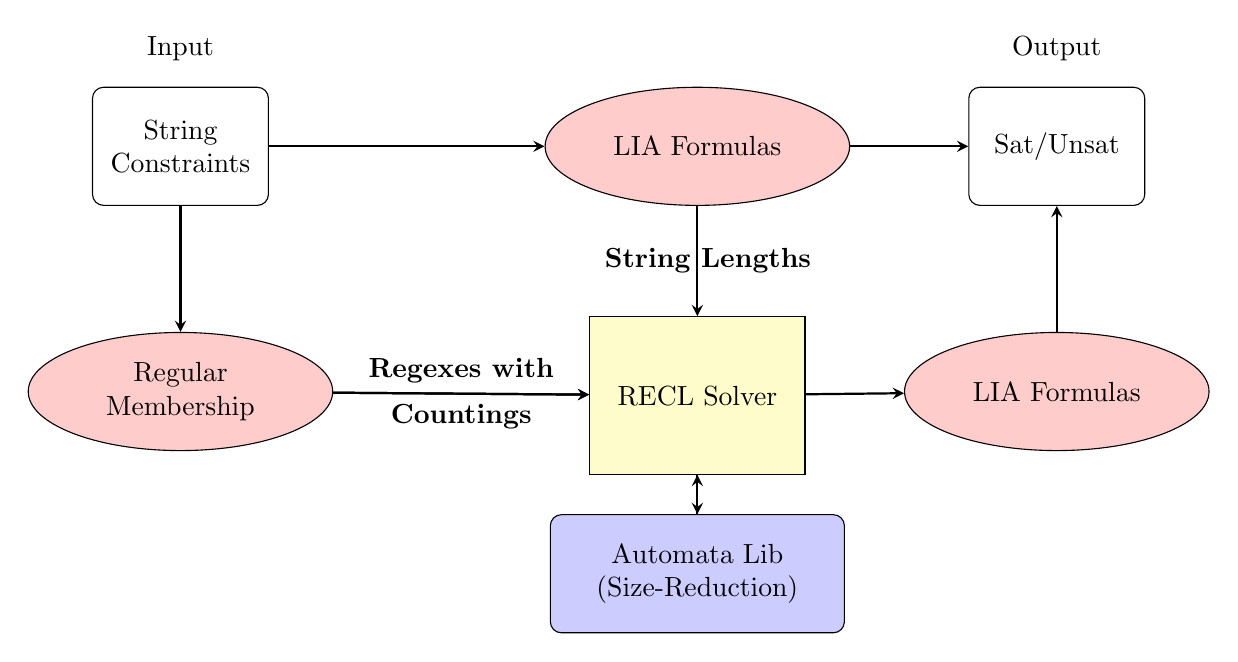
\begin{tikzpicture}[>=latex]

        % Define block styles
        \tikzstyle{input} = [rectangle, draw, fill=white!20, text width=2cm, text centered, rounded corners, minimum height=1.5cm]
        \tikzstyle{output} = [rectangle, draw, fill=white!20, text width=2cm, text centered, rounded corners, minimum height=1.5cm]
        \tikzstyle{component} = [rectangle, draw, fill=blue!20, text width=3.5cm, text centered, rounded corners, minimum height=1.5cm]
        \tikzstyle{core} = [rectangle, draw, fill=yellow!20, text width=2.5cm, text centered, minimum height=2cm]
        \tikzstyle{logic} = [ellipse, draw, fill=red!20, text width=2.5cm, text centered, minimum height=1.5cm]
        \tikzstyle{file} = [rectangle, draw, fill=green!20, text width=1.5cm, text centered, rounded corners, minimum height=1cm]
        \tikzstyle{arrow} = [thick,->,>=stealth]

        % Components
        \node (input) [input] {String Constraints};
        \node (integer) [logic, right=3.5cm of input] {LIA Formulas};
        \node (string) [logic, below=1.6cm of input] {Regular Membership};
        \node (core) [core, below=1.4cm of integer] {RECL Solver};
        \node (output) [output, right=1.5cm of integer] {Sat/Unsat};
        \node (automata) [component, below=.5cm of core] {Automata Lib \\ (Size-Reduction)};
        \node (integer2) [logic, below=1.6cm of output] {LIA Formulas};


        % Arrows
        \draw [arrow] (input) -- (integer);
        \draw [arrow] (integer) to node [midway] {\textbf{\ \ String Lengths}} (core);
        \draw [arrow] (input) -- (string);
        \draw [arrow] (string) to node[midway, above] {\textbf{Regexes with}} (core);
        \draw [arrow] (string) to node[midway, below] {\textbf{Countings}} (core);
        \draw [arrow] (integer) -- (output);
        \draw [arrow] (automata) -- (core);
        \draw [arrow] (core) -- (automata);
        \draw [arrow] (core) -- (integer2);
        \draw [arrow] (integer2) -- (output);

        % Labels
        \node [above=0.2cm of input] {Input};
        \node [above=0.2cm of output] {Output};

      \end{tikzpicture}
    }
  \end{figure}

\end{frame}

\begin{frame}{Benchmark Suites and Environment}
  \begin{benchmark}
    \begin{itemize}
      \item \textbf{RegCoL:} 40,628 instances that contain regexes from real-world websites and are manually constructed.
      \item \textbf{AutomatArk:}  8,215 instances that are adapted from the AutomatArk suite.
    \end{itemize}
  \end{benchmark}
\end{frame}

\begin{frame}{Benchmark Suites and Environment}
  \begin{distribution}
    \includegraphics[width=\linewidth]{counting_distribution.png}
  \end{distribution}
\end{frame}

\begin{frame}{Benchmark Suites and Environment}
  \begin{environment}
    \begin{itemize}
      \item \textbf{Operating System: } CentOS Stream release 8
      \item \textbf{CPU: } Intel(R) Xeon(R) Platinum 8269CY 3.10GHz
      \item \textbf{Memory: } 190 GB
      \item \textbf{Timeout Limit: } 60s
    \end{itemize}
  \end{environment}
\end{frame}

\begin{frame}{Our Solver Solve the Most Instances}
  \centering
  \usepgfplotslibrary{fillbetween}
\pgfplotsset{compat=1.16}
\resizebox{.95\textwidth}{!}{\begin{tabular}{|>{\centering\arraybackslash}m{1.45cm} |c |c |c |c |c |c |}
            \hline
                                                     & CVC5       & Z3str3RE      & Z3str3 & Z3seq & \textsc{Ostrich} & $\ostrichrecl$ \\
            \hline
            \hline

            \rowcolor{grayshade} sat                 & 27813      & 28283         & 23126  & 27761 & 25975            & \textbf{28360} \\
            \hline
            \rowcolor{grayshade} unsat               & 16941      & 19312         & 12742  & 18651 & 20291            & \textbf{20302} \\
            \hline
            \hline

            unknown                                  & \textbf{8} & 99           & 6990   & 98    & 160              & 28             \\
            \hline
            timeout                                  & 4081       & 1149          & 5985   & 2333  & 2417             & \textbf{153}   \\
            \hline
            soundness  error                         & \textbf{0} & 44            & 44     & 56    & \textbf{0}       & \textbf{0}     \\
            \hline
            \hline
            \rowcolor{grayshade} Total\quad  correct & 44754      & 47551         & 35824  & 46356 & 46266            & \textbf{48662} \\
            \hline
            \rowcolor{grayshade} Average  time (s)   & 5.64       & \textbf{1.62} & 7.63   & 3.59  & 5.94             & 1.93           \\
            \hline
      \end{tabular}}
\end{frame}

\begin{frame}{When the Counting Bounds are Large ($\geq 50$)}
  \centering
  \usepgfplotslibrary{fillbetween}
\pgfplotsset{compat=1.16}
\resizebox{.95\textwidth}{!}{\begin{tabular}{|>{\centering\arraybackslash}m{1.45cm} |c |c |c |c |c |c |}
    \hline
                                              & CVC5       & Z3str3RE   & Z3str3     & Z3seq      & \textsc{ostrich} & $\ostrichrecl$ \\
    \hline\hline
    \rowcolor{grayshade} sat                  & 317        & 827        & 616        & 346        & 488              & \textbf{909}   \\
    \hline
    \rowcolor{grayshade} unsat                & 609        & 768        & 694        & 890        & 862              & \textbf{964}   \\
    \hline
    \hline
    unknown                                   & \textbf{1} & 11         & 297        & 11         & 123              & 14             \\
    \hline
    timeout                                   & 1042       & 363        & 362        & 722        & 496              & \textbf{82}    \\
    \hline
    soundness error                           & \textbf{0} & \textbf{0} & \textbf{0} & \textbf{0} & \textbf{0}       & \textbf{0}     \\
    \hline
    \hline
    \rowcolor{grayshade} solved  \quad correctly & 926        & 1595       & 1310       & 1236       & 1350             & \textbf{1873}  \\
    \hline
    \rowcolor{grayshade} average time (s)     & 34.16      & 14.48      & 13.15      & 26.49      & 19.85            & \textbf{5.03}  \\
    \hline
  \end{tabular}}
\end{frame}

\begin{frame}{Justification of Our Technical Choices}
  \centering
  \usepgfplotslibrary{fillbetween}
\pgfplotsset{compat=1.16}
\resizebox{.95\textwidth}{!}{\begin{tabular}{|>{\centering\arraybackslash}m{1.45cm} |c |c |c |}
    \hline
                                              & $\ostrichrecl_{\rm -SIMP}$ & $\ostrichrecl_{\rm NUXMV}$ & $\ostrichrecl$ \\
    \hline\hline
    \rowcolor{grayshade} sat                  & 26884                      & 26603                      & \textbf{28360} \\
    \hline
    \rowcolor{grayshade} unsat                & 20275                      & 20261                      & \textbf{20302} \\
    \hline
    \hline
    unknown                                   & 48                         & 45                         & \textbf{28}    \\
    \hline
    timeout                                   & 1637                       & 1935                       & \textbf{153}   \\
    \hline
    soundness error                           & \textbf{0}                 & \textbf{0}                 & \textbf{0}     \\
    \hline
    \hline
    \rowcolor{grayshade} Total  \quad correct & 47159                      & 46864                      & \textbf{48662} \\
    \hline
    \rowcolor{grayshade} Average  time (s)    & 4.27                       & 6.05                       & \textbf{1.93}  \\
    \hline
  \end{tabular}}
\end{frame}

% Summary and Future work (1min)
% 1 contribution again and main points
% 2 how to handle non-register-representable counting
% 3 potential application 
\section{Conclusion and Future Work}
\begin{frame}
  \frametitle{Our Contributions}
  \begin{enumerate}
    \item Divise an algorithm that efficiently solves string constraints with regex-counting and string-length
    \item Propose particular size-reduction techniquesniques for automata
    \item Carry out extensive experiments
  \end{enumerate}
\end{frame}


\begin{frame}
  \frametitle{Future Work}
  \begin{enumerate}
    \item Symbolically encode non-register-representable counting operators, such as $(a^{\{1,3\}})^*$ and $\overline{a^{\{1,3\}}}$.
    \item Apply this method in generating attack strings of ReDos attack.
  \end{enumerate}
\end{frame}

\end{document}